\documentclass[12pt,a4paper]{article}
\usepackage[utf8]{inputenc}
\usepackage[russian]{babel}
\usepackage[OT1]{fontenc}
\usepackage{mathtools}
\usepackage{amsfonts}
\usepackage{amssymb}
\usepackage{enumitem}
\usepackage{alltt}
\usepackage{graphicx}
\usepackage{indentfirst}
\usepackage{caption}
\usepackage{float}
\usepackage{wrapfig}
\usepackage{physics}
\usepackage{multirow}
\usepackage{longtable}
\usepackage{amsmath,amsfonts,amssymb,amsthm,mathtools}
\usepackage{icomma}
\setlength{\parindent}{0.75cm}
\graphicspath{{pictures/}}
\DeclareGraphicsExtensions{.png}
\usepackage[left=15mm,right=15mm,top=2cm,bottom=2cm]{geometry}
\author{Глотов Алексей}
\begin{document}
\newpage
\begin{center}
\footnotesize{{ГОСУДАРСТВЕННОЕ АВТОНОМНОЕ ОБРАЗОВАТЕЛЬНОЕ УЧРЕЖДЕНИЕ}\break
{ВЫСШЕГО ОБРАЗОВАНИЯ}
\break
{\bf {МОСКОВСКИЙ ФИЗИКО-ТЕХНИЧЕСКИЙ ИНСТИТУТ}}
\break
\small{(НАЦИОНАЛЬНЫЙ ИССЛЕДОВАТЕЛЬСКИЙ УНИВЕРСИТЕТ)}}
\break
\hfill \break
\hfill \break
\begin{center}
\normalsize{Кафедра общей физики}
\end{center}
\hfill \break
\hfill \break
\hfill \break
\hfill \break

\begin{center}
\normalsize {Лабораторная работа 2.1.4}
\end{center}
\hfill \break\\
\large{\textbf{Определение теплоемкости твердых тел}}
\end{center}
\begin{flushleft}
\hfill \break
\hfill \break
\hfill \break
\hfill \break
\hfill \break
\hfill \break
\hfill \break
\hfill \break
\hfill \break
\hfill \break
\hangindent=9cm
\normalsize{Преподаватель:}\hfill
\normalsize{доцент Игуманов А.Ю.}\\
\hfill \break
\normalsize{Обучающийся:}\hfill
\normalsize{Глотов А.А} \\
\hfill \break
\end{flushleft}
\hfill \break
\hfill \break
\hfill \break
\hfill \break
\hfill \break
\hfill \break
\hfill \break
\hfill \break
\hfill \break
\hfill \break
\hfill \break

\begin{center}
Долгопрудный \break
 2022
\end{center}
\thispagestyle{empty}

\newpage

\section{Введение}
\subsection{Аннотация}

Данная работа посвящена изучению явления нагрева твердых тел и определению их теплоемкости. Используются следующие методы: анализ и сведение к полиномиальной функции графиков зависимости R(t), их экстраполяция к нулевой точке. Зависимость сопротивления от времени снимается с помощью электронных омметра и секундомера 

\textbf{Цель работы:}  \begin{enumerate}
	\item  измерение количества подведенного тепла и вызванного им нагрева твердого тела
	\item определение теплоемкости по экстраполяции отношения $\Delta{Q}/\Delta{T}$ к нулевым потерям тепла
\end{enumerate}

\textbf{Приборы и материалы:}
\begin{itemize}
	\item калориметр с нагревателем и термометром сопротивления
	\item амперметр
	\item вольтметр
	\item мост постоянного тока
	\item источник питания 36 В
\end{itemize}


\subsection{Теоретические сведения}

В данной работе происходит измерение теплоемкости твердого тела с использованием следующей принципиальной связи:
	
	\begin{equation}
		C = \frac{\Delta Q}{\Delta T}
		\label{eq:first_eq_of_thermal_capacity}
	\end{equation}
	
	Определение количества теплоты, переданного телу вызывает некоторые затруднения, так как часть теплоты будет передано окружающей среде через стенки калориметра. В итоге, количество теплоты, переданное телу с учетом теплопотерь через стенки можно определить как:
	
	\begin{equation}
		\Delta Q = P\Delta t - \lambda \left( T - T_{\text{к}} \right) \Delta t,
		\label{eq:termal_with_heat_lossing}
	\end{equation}
	 где $P$ -- мощность нагревателя, $\lambda$ -- коэффициент теплоотдачи стенок калориметра, $T$ -- температура тела, $T_{\text{к}}$ -- температура окружающего калориметр воздуха, $\Delta t$ -- время, в течении которого происходит нагрев.
	 
	 Из уравнений (\ref{eq:first_eq_of_thermal_capacity}) и (\ref{eq:second_eq_of_thremal_capacity}) получаем:
	 
	 \begin{equation}
	 	C = \frac{P - \lambda \left(T - T_{\text{к}} \right) }{\Delta T /\Delta t}
	 	\label{eq:second_eq_of_thremal_capacity}
	 \end{equation}
	 
	Формула (\ref{eq:second_eq_of_thremal_capacity}) является основной расчетной формулой данной работы.
	
\subsection{Схема эксперимента}

 При неизменной мощности нагревателя определим зависимость сопротивления термометра от времени для пустого калориметра
Для этого сначала сбалансируем мост. Замкнем цепь нагревателя и одновременно включим секундомер. Установим на мосте постоянного тока сопротивление, немного большее (на
0,5\%), чем это необходимо для балансировки (стрелка гальванометра при этом отклонится от нулевого значения).
В тот момент, когда сопротивление термометра возрастет до значения, установленного на мосте, и балансировка восстановится, отметим показания секундомера. Затем вновь увеличим сопротивление на мосте и отметим время восстановления балансировки и т. д. Таким образом получим 10–15 точек. 

Охладим калориметр до исходной температуры. Поместим туда исследуемое тело и проведем аналогичную серию измерений. Повторим вышеописанные действия для каждого из трех исследуемых конусов. По полученным четырем наборам точек построим графики зависимости R(t) и проведем плавные кривые.

Определим полиномиальные уравнения этих кривых, а затем по этим данных - уравнение касательных к ним. Экстраполируем графики полученных уравнений к точке нулевых потерь тепла

Определим теплоемкости исследуемых систем "калориметр + конус" и пустого калориметра. По разности значений определим значения теплоемкостей наших конусов.

\subsection{Методика измерений}


	В формуле (\ref{eq:second_eq_of_thremal_capacity}) в знаменателе стоит величина, для определения которой воспользуемся следующей методикой:
	
	Построим график зависимости $\frac{\Delta T}{\Delta t} = f \left( T \right)$ для широкого диапазона температур, после чего экстраполируем его для значения $T = T_{\text{к}}$. В таком случае формула (\ref{eq:second_eq_of_thremal_capacity}) приобретает вид:
	
	\begin{equation}
		C = \frac{P}{\left( \Delta T / \Delta t \right)_{T_{\text{к}}}}
		\label{eq:final_eq_for_capacity}
	\end{equation}
	
	Измерение температуры строится на принципе линейной зависимости сопротивления материала от изменения температуры по закону:
	
	\begin{equation}
		R_{T} = R_{0} \left( 1 + \alpha \Delta T \right),
	\end{equation}
	
	Где $R_{0}$ -- сопротивление термометра при комнатной температуры, $R_{T}$ -- сопротивление термометра при данной температуре. Учитывая данную зависимость, получаем итоговый вид для основной формулы:
	
	\begin{equation}
		C = \frac{PR\alpha}{\left( \frac{dR}{dt} \right)_{T_{\text{к}}}\left( 1 + \alpha \Delta T_{\text{К}} \right)}
		\label{eq:capacity}
	\end{equation}	 
	
	Коэффициент $\alpha$, входящий в данную формулу для меди равен $\alpha = 4,28 \cdot 10^{-3} \, K^{-1}$, все остальные величины определяются экспериментально.



\subsection{Экспериментальная установка}

	
	\begin{wrapfigure}[9]{r}{0.3\textwidth}
		\vspace{-2.5ex}
		\begin{center}
			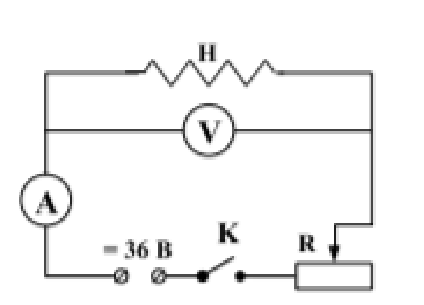
\includegraphics[width = 0.2\textwidth]{2.1.4_1}
			\caption{Схема установки}
			\label{fig:schem_of_facility}
		\end{center}
	\end{wrapfigure}

	Установка состоит из калориметра с пенопластовой изоляцией, помещенного в ящик из многослойной клееной фанеры. Внутренние стенки калориметра выполнены из материала с высокой теплопроводностью. Надежность теплового контакта между телом и стенками обеспечивается их формой: они имеют форму усеченных конусов и плотно прилегают друг к другу. Для выталкивания образца служит винт в донышке внутренней стенки калориметра.
	
	В стенку калориметра вмонтированы электронагреватель и термометр сопротивления. Схема включения нагревателя изображена на рисунке (\ref{fig:schem_of_facility}). Система реостатов позволяет установить нужную силу тока в цепи нагревателя. По амперметру и вольтметру определяется мощность, выделяемая током в нагревателе. Величина сопротивления термометра нагревателя  измеряется мостом постоянного тока.
	
	\begin{figure}[h!]
		\begin{center}
			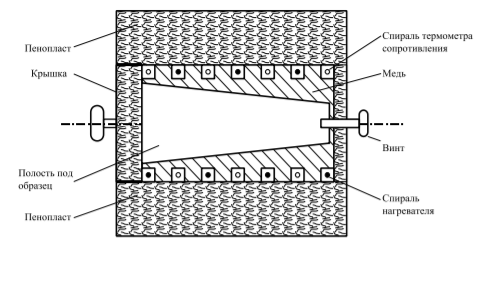
\includegraphics[width = 0.5\textwidth]{2.1.4_2}
			\caption{Устройство калориметра}
			\label{fig:Ris_of_facility}
		\end{center}
	\end{figure}

	На рисунке изображено устройство калориметра.
	
	Запишем также иные параметры экспериментальной установки
	
	\begin{table}[h!]
		\centering
		\begin{tabular}{|c|c|c|c|}
			\hline
			материал образца: & железо          & латунь          & алюминий        \\ \hline
			масса образца, г  & $813,2 \pm 0,1$ & $868,7 \pm 0,1$ & $294,2 \pm 0,1$ \\ \hline
		\end{tabular}
		\caption{Параметры исследуемых образцов}
		\label{tab:param_of_facility}
	\end{table}
	
	$$R_{0} = 17,73 \pm 0,01 \, \text{Ом}, P = 10.8\text{Вт}$$

\newpage

\section{Результаты измерений и обработка данных}

Снимем зависимость R(t) и занесем полученные данные в таблицу
\begin{center}
\begin{tabular}{|c|c|c|c|c|c|c|c|}
\hline 
\multicolumn{2}{|c|}{Enemy} & \multicolumn{2}{|c|}{Fe} & \multicolumn{2}{|c|}{L} & \multicolumn{2}{|c|}{Al} \\ 
\hline 
\multicolumn{2}{|c|}{$T_{0} = 292.4 K$} & \multicolumn{2}{|c|}{$T_{0} = 293.2 K$} & \multicolumn{2}{|c|}{$T_{0} = 295.8 K$} & \multicolumn{2}{|c|}{$T_{0} = 297.0 K$} \\ 
\hline 
R, Ом & t, с & R, Ом & t, с & R, Ом & t, с & R, Ом & t, с \\ 
\hline 
17.730 & 0 & 17.679 & 0 & 17.722 & 0 & 17.805 & 0 \\ 
\hline 
17.780 & 34 & 17.747 & 39 & 17.772 & 40 & 17.855 & 44 \\ 
\hline 
17.830 & 79 & 17.797 & 104 & 17.822 & 94 & 17.905 & 101 \\ 
\hline 
17.880 & 124 & 17.847 & 172 & 17.872 & 160 & 17.955 & 161 \\ 
\hline 
17.930 & 170 & 17.897 & 242 & 17.922 & 223 & 18.005 & 227 \\ 
\hline 
17.980 & 220 & 17.947 & 315 & 17.972 & 294 & 18.055 & 293 \\ 
\hline 
18.030 & 270 & 17.997 & 391 & 18.022 & 365 & 18.105 & 361 \\ 
\hline 
18.080 & 321 & 18.047 & 470 & 18.072 & 439 & 18.155 & 427 \\ 
\hline 
18.130 & 374 & 18.097 & 546 & 18.122 & 511 & 18.205 & 498 \\ 
\hline 
18.180 & 429 & 18.147 & 628 & 18.172 & 590 & 18.255 & 570 \\ 
\hline 
18.230 & 486 & 18.197 & 710 & 18.222 & 667 & 18.305 & 645 \\ 
\hline 
18.280 & 545 & 18.247 & 796 & 18.272 & 749 & 18.355 & 719 \\ 
\hline 
18.330 & 605 & 18.297 & 884 & 18.322 & 831 & 18.405 & 797 \\ 
\hline 
18.380 & 665 & 18.347 & 973 & 18.372 & 918 & 18.455 & 875 \\ 
\hline 
18.430 & 729 & 18.397 & 1065 & 18.422 & 1008 & 18.505 & 956 \\ 
\hline 
\end{tabular} 
\end{center}

По полученным точкам построим графики зависимостей R(t). Для наглядности сдвинем их все в точку (0;0)

\begin{figure}[H]
	\begin{center}
		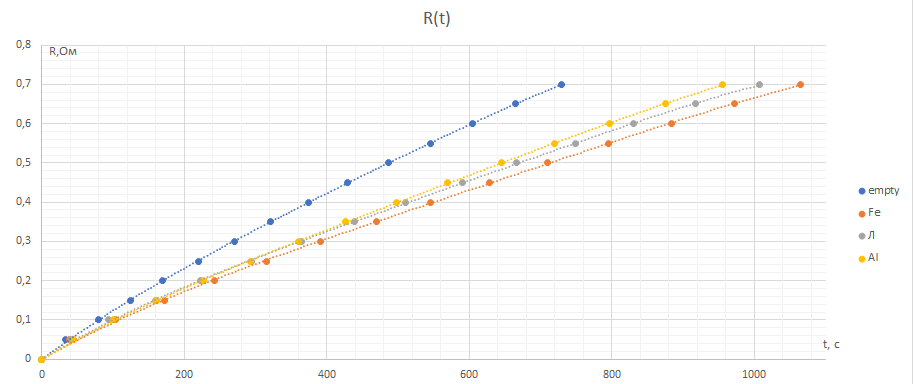
\includegraphics[width=14cm]{2.1.4_gr_1}
	\end{center}
\end{figure}

Приведем приближенные уравнения каждой из наших кривых.\hfill \break
enemy: $R = -8*10^{-13}*t^4 + 2*10^{-9}*t^3 - 1*10^{-6}*t^2 + 0,0013*t + 17.73$ \hfill \break
Fe: $R = -4*10^{-13}*t^4 + 1*10^{-9}*t^3 - 1*10^{-6}*t^2 + 0,001*t + 17.679$ \hfill \break
L: $R = -6*10^{-13}*t^4 + 1*10^{-9}*t^3 - 1*10^{-6}*t^2 + 0,0011*t + 17.722$ \hfill \break
Al: $R = -5*10^{-13}*t^4 + 1*10^{-9}*t^3 - 9*10^{-7}*t^2 + 0,001*t + 17.805$

Продиффиринцируем наши уравнения и подставим полученные ранее значения времени, таким образом по полученным точкам построим и определим уравнение зависимости $\frac{dR}{dt}(R)$. Из-за очевидности преобразований, зафиксируем здесь только конечные точки и полученные уравнения.

\begin{center}
\begin{tabular}{|c|c|c|c|c|c|c|c|}
\hline 
\multicolumn{2}{|c|}{Enemy} & \multicolumn{2}{|c|}{Fe} & \multicolumn{2}{|c|}{L} & \multicolumn{2}{|c|}{Al} \\ 
\hline  
$\frac{dR}{dt}, \frac{\text{Ом}}{c}*10^{-4}$ & R, Ом & $\frac{dR}{dt}, \frac{\text{Ом}}{c}*10^{-4}$ & R, Ом & $\frac{dR}{dt}, \frac{\text{Ом}}{c}*10^{-4}$ & R, Ом & $\frac{dR}{dt}, \frac{\text{Ом}}{c}*10^{-4}$ & R, Ом \\ 
\hline 
13.4 & 17.730 & 10.2 & 17.679 & 11.1 & 17.722 & 10.5 & 17.805 \\ 
\hline 
12.7 & 17.780 & 9.5 & 17.747 & 10.2 & 17.772 & 9.7 & 17.855 \\ 
\hline 
11.8 & 17.830 & 8.5 & 17.797 & 9.2 & 17.822 & 9.0 & 17.905 \\ 
\hline 
11.1 & 17.880 & 7.7 & 17.847 & 8.2 & 17.872 & 8.3 & 17.955 \\ 
\hline 
10.5 & 17.930 & 7.0 & 17.897 & 7.5 & 17.922 & 7.8 & 18.005 \\ 
\hline 
10.0 & 17.980 & 6.6 & 17.947 & 7.0 & 17.972 & 7.4 & 18.055 \\ 
\hline 
9.7 & 18.030 & 6.3 & 17.997 & 6.7 & 18.022 & 7.2 & 18.105 \\ 
\hline 
9.4 & 18.080 & 6.2 & 18.047 & 6.5 & 18.072 & 7.0 & 18.155 \\ 
\hline 
9.2 & 18.130 & 6.1 & 18.097 & 6.5 & 18.122 & 6.9 & 18.205 \\ 
\hline 
9.0 & 18.180 & 6.1 & 18.147 & 6.5 & 18.172 & 6.9 & 18.255 \\ 
\hline 
8.8 & 18.230 & 6.1 & 18.197 & 6.4 & 18.222 & 6.8 & 18.305 \\ 
\hline 
8.6 & 18.280 & 6.0 & 18.247 & 6.3 & 18.272 & 6.7 & 18.355 \\ 
\hline 
8.3 & 18.330 & 5.8 & 18.297 & 6.1 & 18.322 & 6.5 & 18.405 \\ 
\hline 
8.0 & 18.380 & 5.3 & 18.347 & 5.5 & 18.372 & 6.1 & 18.455 \\ 
\hline 
7.4 & 18.430 & 4.6 & 18.397 & 4.6 & 18.422 & 5.5 & 18.505 \\ 
\hline 
\end{tabular} 
\end{center}

Запишем получившиеся уравнения (приблизительные) $\frac{dR}{dt}(R)$: \hfill \break
enemy: $\frac{dR}{dt}(R) = -0.0047*R^4 + 0.3359*R^3 - 9.0314*R^2 + 107.8968*R - 487.2627$ \hfill \break
Fe: $\frac{dR}{dt}(R) = -0.0092*R^4 + 0.6558*R^3 - 17.6176*R^2 + 210.3259*R - 941.4295$ \hfill \break
L: $\frac{dR}{dt}(R) = -0.0112*R^4 + 0.8022*R^3 - 21.5944*R^2 + 258.3006*R - 1158.4233$ \hfill \break
Al: $\frac{dR}{dt}(R) = -0.0059x4 + 0.4233x3 - 11.4197x2 + 136.9071x - 615.3561$

Экстраполируем наш график к точке, где потери тепла нулевые, т.е. в точку, где температура системы равна комнатной (точка начального сопротивления)

\begin{table}[h!]
		\centering
		\begin{tabular}{|c|c|c|c|c|}
			\hline
			эксперимент: & enemy & Fe & L & Al \\ \hline
			 $\frac{dR}{dt}(R), \frac{\text{Ом}}{c} * 10^{-4}$  & 12.22 & 8.30 & 9.43 & 10.56 \\ \hline
		\end{tabular}
	\end{table}

Теперь по формуле (6) определим теплоемкости наших систем

\begin{table}[h!]
		\centering
		\begin{tabular}{|c|c|c|c|c|}
			\hline
			эксперимент: & enemy & Fe & L & Al \\ \hline
			 $C, \frac{\text{Дж}}{K}$  & 669.5 & 1039.2 & 971.7 & 886.7 \\ \hline
		\end{tabular}
	\end{table}

Зная, что полученные теплоемкости - сумма теплоемкостей калориметра и нашего тела, посчитаем удельные теплоемкости.

Погрешности наших измерений складываются из случайной и систематической. В нашем случае, систематическая погрешность мала, а случайная определяется погрешностями экстраполяции. С помощью специализированных программ определим ее.

\begin{table}[h!]
		\centering
		\begin{tabular}{|c|c|c|c|c|}
			\hline
			эксперимент: & enemy & Fe & L & Al \\ \hline
			 $c, \frac{\text{Дж}}{\text{кг}*K}$ & - & 454.6 & 347.9 & 738.3 \\ \hline
			 относительная погрешность: & 0.011 & 0.007 & 0.005 & 0.009 \\ \hline
		\end{tabular}
	\end{table}

Тогда итоговые значения теплоемкостей:

$c_{Fe} = (455 \pm 8)\frac{\text{Дж}}{\text{кг}*K}$

$c_{L} = (347 \pm 6)\frac{\text{Дж}}{\text{кг}*K}$

$c_{Fe} = (738 \pm 15)\frac{\text{Дж}}{\text{кг}*K}$

\newpage

\section{Обсуждение результатов и выводы}
В ходе работы были достигнуты следующие цели:
\begin{itemize}
\item Зафиксирована зависимость сопротивления калориметра в зависимости от его температуры и содержимого
\item Экспериментально получены значения теплоемкостей исследуемых твердых тел и удельных теплоемкостей материалов, из которых они были изготовлены, а также калориметра  
\end{itemize}

Значения теплоемкостей получены с довольно неплохой точностью (до 2\%), что объясняется малой погрешностью измерительных приборов, а также компьютизированными методами обработки данных, которые позволили установить максимально подходящие функции под полученные точки.  

Итоговые значения удельных теплоемкостей также получены с неплохой точностью. Однако удовлетворительным можно считать только результат измерений для железного тела ($(455 \pm 8)\frac{\text{Дж}}{\text{кг}*K}$ - эксперимент и 440 $\frac{\text{Дж}}{\text{кг}*K}$ - табличное значение). Для латунного ($(347 \pm 6)\frac{\text{Дж}}{\text{кг}*K}$ - эксперимент и 400 $\frac{\text{Дж}}{\text{кг}*K}$ - табличное значение) алюминиевого ($(738 \pm 15)\frac{\text{Дж}}{\text{кг}*K}$ - эксперимент и 920 $\frac{\text{Дж}}{\text{кг}*K}$ - табличное значение) образцов результат нельзя считать приемлемым. 

В связи с большим расхождением двух из трех результатов с табличными значениями, можно сделать несколько выводов. Во-первых, предложенный метод ручной обработки данных с помощью построения касательных не оправдан. При его использовании погрешность увеличилась бы многократно, а лучший результат можно было бы получить только случайным образом. Во-вторых,следует задуматься о перепроверке результатов с другими образцами и на других установках. Если результат повторится - это будет говорить о крайне низкой точности метода. Если ошибка будет исключена, то можно будет утверждать о неисправности установки 

\end{document}